% Free range VHDL
% Authors: Bryan Mealy, Fabrizio Tappero
% Date: May, 2012
% URL: freerangefactory.org
% (C) 2013 B. Mealy, F. Tappero
%
% !TEX root = master.tex
%
\chapter{Finite State Machine Design Using VHDL}
Finite state machines (FSMs) are mathematical abstractions that are used to solve a large variety of problems, among which are electronic design automation, communication protocol design, parsing and other engineering applications. At this point in your digital design career, you might have probably designed quite a few state machines on paper. You are now at the point where you can implement and test them using actual hardware if you so choose. The first step in this process is to learn how to model FSMs using VHDL. 

As you will see in the next section, simple FSM designs are just a step beyond the sequential circuit design described in the previous section. The techniques you learn in this section will allow you to quickly and easily design relatively complex FSMs which can be very useful in many number of ways.

\begin{figure}
    \centering
	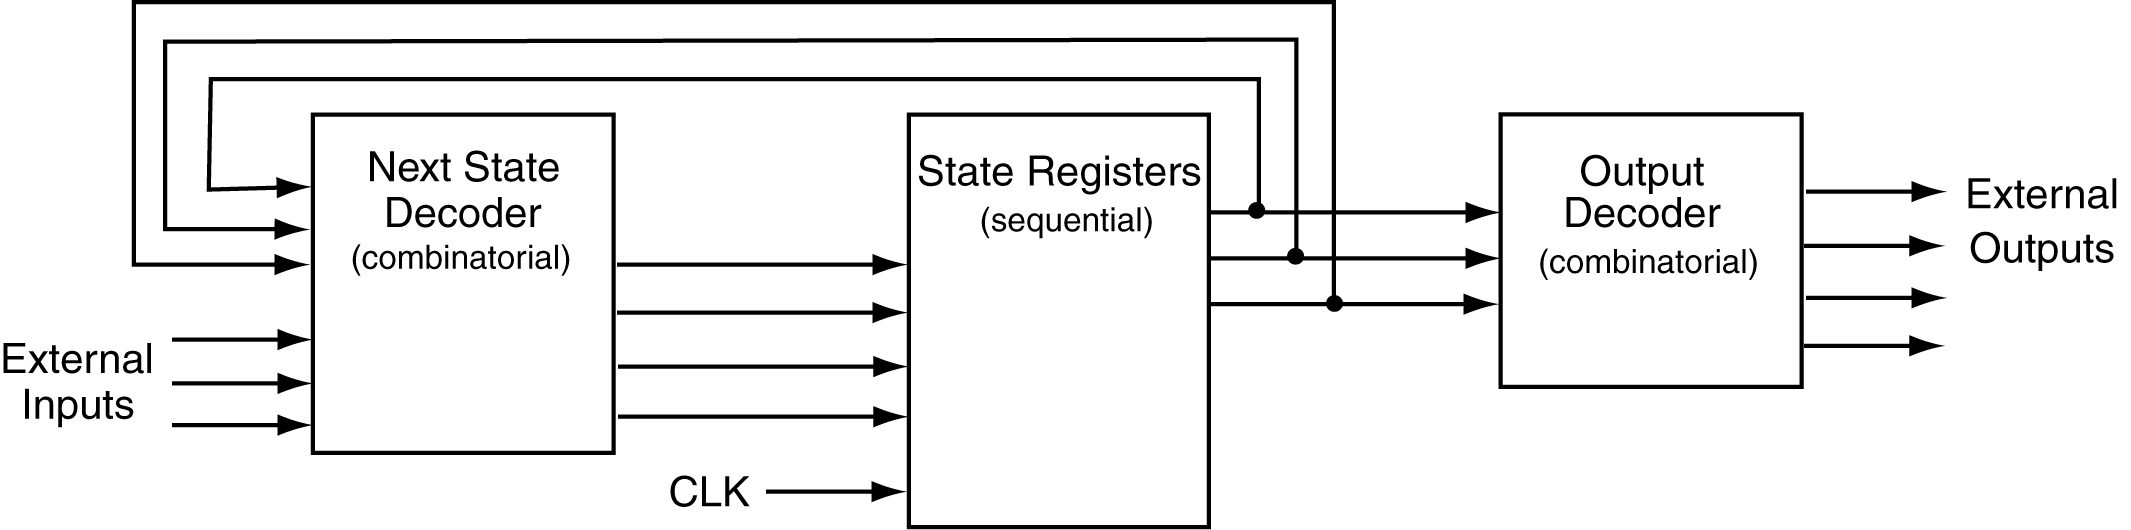
\includegraphics[width=13cm]{fsm/fsm.png}
	\caption{Block diagram for a Moore-type FSM.}
	\label{fsm}
\end{figure}

A block diagram for a standard Moore-type FSM is shown in Fig.~\ref{fsm}. This diagram looks fairly typical but different names are used for some of the blocks in the design. The \texttt{Next State Decoder} is a block of combinatorial logic that uses the current external inputs and the current state to decide upon the next state of the FSM. In other words, the inputs to the \texttt{Next State Decoder} block are decoded to produce an output that represents the next state of the FSM. The circuitry in \texttt{Next State Decoder} is generally the excitation equations for the storage elements (flip-flops) in the \texttt{State Register} block. The next state becomes the present state of the FSM when the clock input to the state registers block becomes active. The state registers block is a storage element that stores the present state of the machine. The inputs to the \texttt{Output Decoder} are used to generate the desired external outputs. The inputs are decoded via combinatorial logic to produce the external outputs. Because the external outputs are only dependent upon the current state of the machine, this FSM is classified as a Moore-type FSM.

The FSM model shown in Fig.~\ref{fsm} is probably the most common model for describing a Moore-type FSM. That is most likely because students are often asked to generate the combinatorial logic required to implement the \texttt{Next State Decoder} and the \texttt{Output Decoder}; however here we want to think about FSMs in the context of VHDL. The true power of VHDL starts to emerge in its dealings with FSMs. As you will see, the versatility of VHDL behavioral modeling removes the need for large paper designs of endless K-maps and endless combinatorial logic elements.

\begin{figure}[t]
    \centering
	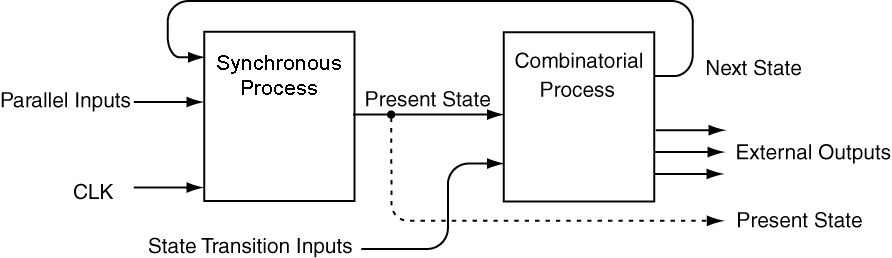
\includegraphics[width=12cm]{fsm/fsm_imp.png}
	\caption{Model for VHDL implementations of FSMs.}
	\label{fsm_imp}
\end{figure}

There are several different approaches used to model FSMs using VHDL. The many different possible approaches are a result of the general versatility of VHDL as a language. What we will describe in this section is probably the clearest approach for FSM implementation. A block diagram of the approach we will use in the implementation of FSMs is shown in Fig.~\ref{fsm_imp}.

Although it does not look that much clearer, you will soon be finding the FSM model shown in Fig.~\ref{fsm_imp} to be a straightforward method to implement FSMs. The approach we will use divides the FSM into two VHDL processes. One process, referred to as the \texttt{Synchronous Process} handles all the matters regarding clocking and other controls associated with the storage element. The other process, the \texttt{Combinatorial Process}, handles all the matters associated with the \texttt{Next State Decoder} and the \texttt{Output Decoder} of Fig.~\ref{fsm}. Note that the two blocks in Fig.~\ref{fsm} are both made solely of combinatorial logic.


There is some new lingo used in the description of signals used in Fig.~\ref{fsm_imp}; this description is outlined and described below: 
\begin{my_list}
\item The inputs labelled \texttt{Parallel Inputs} are used to signify inputs that act in parallel to each of the storage elements. These inputs would include enables, presets, clears, etc. 

\item The inputs labelled \texttt{State Transition Inputs} include external inputs that control the state transitions. These inputs also include external inputs used to decode Mealy-type external outputs. 

\item The \texttt{Present State} signals are used by the \texttt{Combinatorial \\ Process} box for both next state decoding and output decoding. The diagram of Fig.~\ref{fsm_imp} also shows that the \texttt{Present State} variables can also be provided as outputs to the FSM but they are not required.
\end{my_list}

One final comment before we begin. Although there are many different methods that can be used to described FSMs using VHDL, two of the more common approaches are the dependent and independent PS/NS styles. This book only covers the dependent style because it is clearer than the independent PS/NS style. The model shown in Fig.~\ref{fsm_imp} is actually a model of the dependent PS/NS style of FSMs. Once you understand the VHDL modeling of the dependent PS/NS style of FSM, the understanding of the independent PS/NS style or any other style is relatively painless. More information on the other FSM coding styles is found in various VHDL texts or on the web.

\section{VHDL Behavioral Representation of FSMs}

\begin{leftbar}
\begin{minipage}[t]{0.5\textwidth}
\vspace{10pt}
\noindent
\textbf{EXAMPLE 18.}
Write the VHDL code that implements the FSM shown on the right. Use a dependent PS/NS coding style in your implementation.
\end{minipage}
\begin{minipage}[t]{0.47\textwidth}
\vspace{0pt}\raggedright
    \centering
	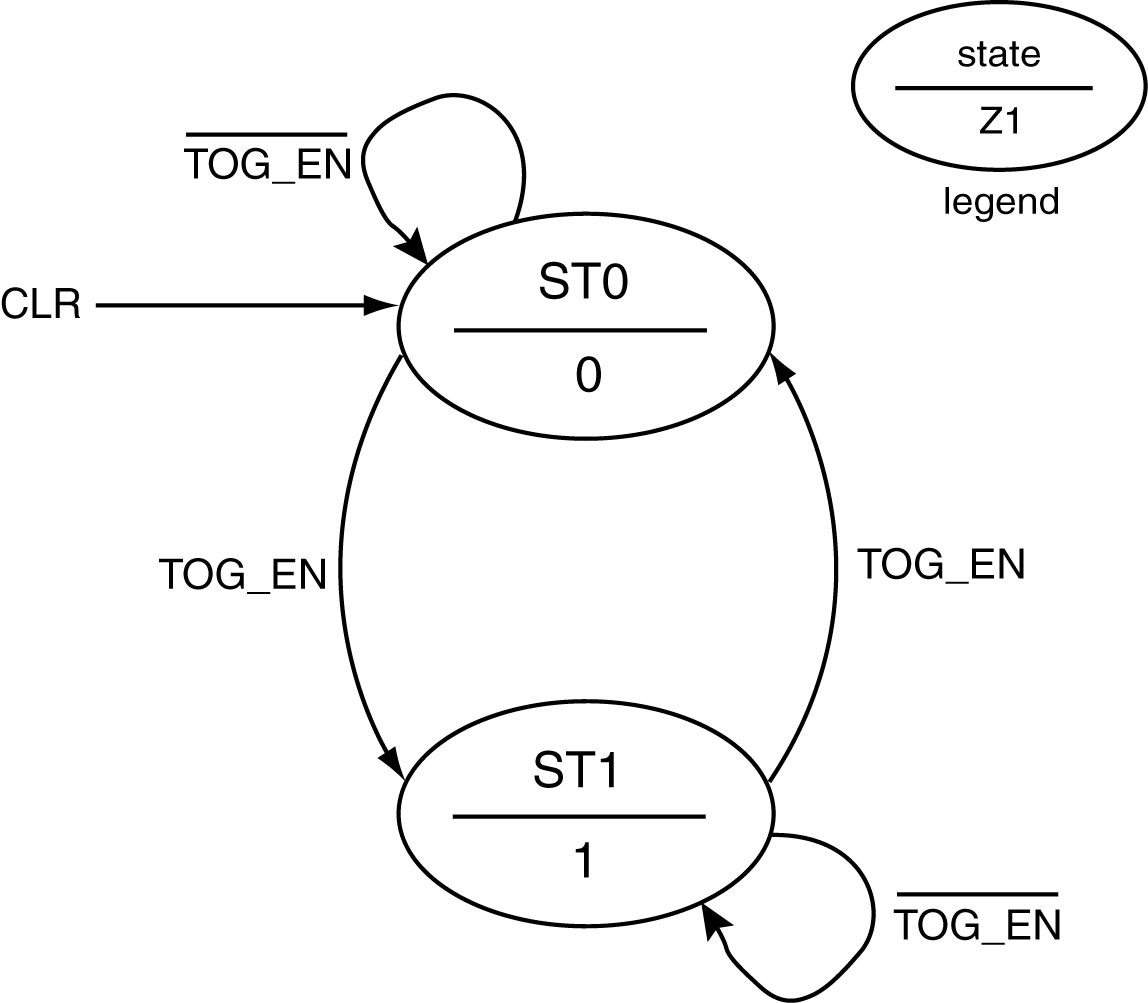
\includegraphics[width=5.3cm]{fsm/ex18.png}
\end{minipage}
\end{leftbar}
\noindent
\textbf{SOLUTION.} This problem represents a basic FSM implementation. It is somewhat instructive to show the black-box diagram which is an aid in writing the entity description. Starting FSM problems with the drawing of a black box diagram is always a healthy approach particularly when dealing with FSMs. Oftentimes with FSM problems, it becomes challenging to discern the FSM inputs from the outputs. Drawing a diagram partially alleviates this problem. The black box diagram and the code for the solution of Example~18 is shown in Listing~\ref{exe_18_code}.

\begin{figure}[!h]
    \centering
	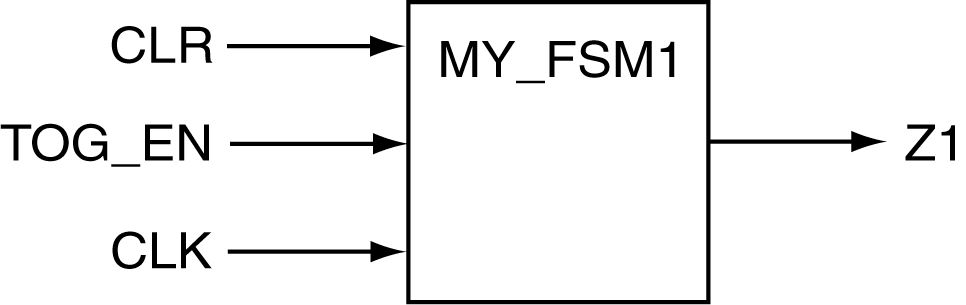
\includegraphics[width=5cm]{fsm/ex18_sol.png}
\end{figure}

\noindent
\begin{minipage}{0.99\linewidth}
\begin{lstlisting}[label=exe_18_code, caption=Solution to Example~18.]
-- library declaration
library IEEE;
use IEEE.std_logic_1164.all;
-- entity
entity my_fsm1 is 
    port (  TOG_EN  : in  std_logic; 
            CLK,CLR : in  std_logic; 
                 Z1 : out std_logic); 
end my_fsm1;
-- architecture
architecture fsm1 of my_fsm1 is
   type state_type is (ST0,ST1); 
   signal PS,NS : state_type; 
begin
   sync_proc: process(CLK,NS,CLR)
   begin
     -- take care of the asynchronous input
     if (CLR = '1') then 
        PS <= ST0;  
     elsif (rising_edge(CLK)) then 
        PS <= NS; 
     end if; 
   end process sync_proc; 

   comb_proc: process(PS,TOG_EN)
   begin
      Z1 <= '0';        -- pre-assign output
      case PS is 
         when ST0 =>    -- items regarding state ST0
            Z1 <= '0';  -- Moore output
            if (TOG_EN = '1') then NS <= ST1; 
            else  NS <= ST0; 
            end if; 
         when ST1 =>    -- items regarding state ST1
            Z1 <= '1';  -- Moore output
            if (TOG_EN = '1') then NS <= ST0; 
            else  NS <= ST1; 
            end if; 
         when others => -- the catch-all condition
            Z1 <= '0';  -- arbitrary; it should never 
            NS <= ST0;  -- make it to these two statements
      end case; 
   end process comb_proc; 
end fsm1;
\end{lstlisting}
\end{minipage}

And of course, this solution has many things worth noting in it. The more interesting things are listed below. 

\begin{my_list}
\item We have declared a special VHDL type named \texttt{state\_type} to represent the states in this FSM. This is an example of how enumeration types are used in VHDL. As with enumeration types in other higher-level computer languages, there are internal numerical representations for the listed state types but we only deal with the more expressive symbolic equivalent. In this case, the type we have created is called a \texttt{state\_type} and we have declared two variables of this type: PS and NS. The key thing to note here is that a \texttt{state\_type} is something we have created and is not a native VHDL type.

\item The synchronous process is equal in form and function to the simple D~flip-flops we examined in the section about sequential circuits. The only difference is that we have substituted PS and NS for D and Q, respectively. Something to note here is that the storage element is associated with the PS signal only. Note that PS is not specified for every possible combination of inputs. 

\item Even though this example is of the simplest FSM you could hope for, the code looks somewhat complicated. But if you examine it closely, you can see that everything is nicely compartmentalized in the solution. There are two processes; the synchronous process handles the asynchronous reset and the assignment of a new state upon the arrival of the system clock. Additionally, the combinational process handles the outputs not handled in the synchronous process. 

\item Because the two processes operate concurrently, they can be considered as working in a lock-step manner. Changes to the NS signal that are generated in the combinatorial process force an evaluation of the synchronous process. When the changes are actually instituted in the synchronous process on the next clock edge, the changes in the PS signal causes the combinatorial process to be evaluated. And so on and so forth. 

\item The case statement in the combinatorial process provides a \texttt{when} clause for each state of the FSM. This is the standard approach for the dependent PS/NS coding style. A \texttt{when others} clause has also been used. The signal assignments that are part this catch-all clause are arbitrary since the code should never actually make it there. This statement is provided for a sense of completeness and represents good VHDL coding practice. 

\item The Moore output is a function of only the present state. This is expressed by the fact that the assignment of the Z1 output is unconditionally evaluated in each when clause of the case statement in the combinatorial process. In other words, the Z1 variable is inside the \texttt{when} clause but outside of the \texttt{if} statement in the \texttt{when} clause. This is of course because the Moore outputs are only a function of the states and not the external inputs. Note that it is the external input that controls the \texttt{which} state the FSM transitions to from any given state. You will see later that Mealy outputs, due their general nature, are assigned inside the \texttt{if} statement.

\item The Z1 output is pre-assigned as the first step in the combinatorial process. Pre-assigning it in this fashion prevents the unexpected latch generation for the Z1 signal. When dealing with FSMs, there is a natural tendency for the FSM designer to forget to specify an output for the Z1 variable in each of the states. Pre-assigning it prevents latches from being generated and can arguably clean up the source code. The pre-assignment makes no difference to the VHDL code because if multiple assignments are made within the code, only the final assignment takes effect. In other words, only the final assignment is considered once the process terminates. 
\end{my_list}

There is one final thing to note about Example~18. In an effort to keep the example simple, we disregarded the digital values of the state variables. This is indicated in the black-box diagram of Listing~\ref{exe_18_code} by the fact that the only output of the FSM is the signal Z1. This is reasonable in that it could be considered that only one output was required in order to control some other device or circuit. The state variable is represented internally and its precise representation is not important since the state variable is not provided as an output. 

In some FSM designs, the state variables are provided as outputs. To show this situation, we will provide a solution to Example~18 with the state variables as outputs. The black-box diagram and the VHDL code of this solution is shown in Listing~\ref{exe_18_code_alt}.
\begin{figure}[!h]
    \centering
	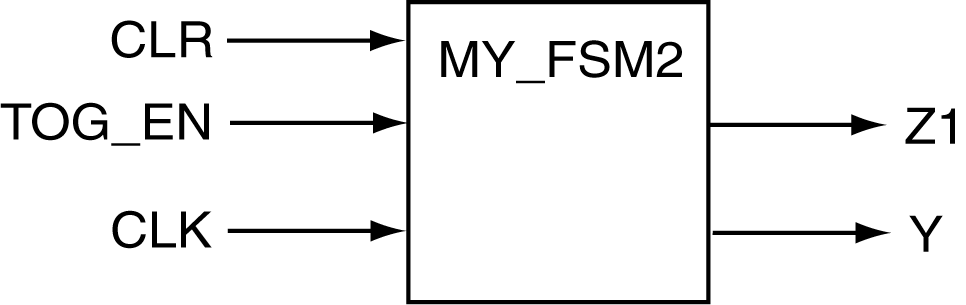
\includegraphics[width=5cm]{fsm/ex18_sol_alt.png}
\end{figure}

\noindent
\begin{minipage}{0.99\linewidth}
\begin{lstlisting}[label=exe_18_code_alt, caption=Solution to Example~18 that include state variable as output.]
-- library declaration
library IEEE;
use IEEE.std_logic_1164.all;
-- entity
entity my_fsm2 is 
   port (   TOG_EN : in  std_logic; 
           CLK,CLR : in  std_logic; 
              Y,Z1 : out std_logic); 
end my_fsm2;
-- architecture
architecture fsm2 of my_fsm2 is
   type state_type is (ST0,ST1); 
   signal PS,NS : state_type; 
begin
   sync_proc: process(CLK,NS,CLR)
   begin
      if (CLR = '1') then 
         PS <= ST0; 
      elsif (rising_edge(CLK)) then 
         PS <= NS; 
      end if; 
   end process sync_proc; 

   comb_proc: process(PS,TOG_EN)
   begin
      Z1 <= '0';
      case PS is    
         when ST0 =>        -- items regarding state ST0
            Z1 <= '0';      -- Moore output
            if (TOG_EN = '1') then NS <= ST1; 
            else  NS <= ST0; 
            end if; 
         when ST1 =>        -- items regarding state ST1
            Z1 <= '1';      -- Moore output
            if (TOG_EN = '1') then NS <= ST0; 
            else  NS <= ST1; 
            end if; 
         when others =>     -- the catch-all condition
            Z1 <= '0';      -- arbitrary; it should never 
            NS <= ST0;      -- make it to these two statements
      end case; 
   end process comb_proc; 
 
   -- assign values representing the state variables
   with PS select
      Y <= '0' when ST0, 
           '1' when ST1, 
           '0' when others; 
end fsm2;
\end{lstlisting}
\end{minipage}

Note that the VHDL code shown in Listing~\ref{exe_18_code_alt} differs in only two areas from the code shown in Listing~\ref{exe_18_code}. The first area is the modification of the entity declaration to account for the state variable output Y. The second area is the inclusion of the selective signal assignment statement which assigns a value of state variable output Y based on the condition of the state variable. The selective signal assignment statement is evaluated each time a change in signal PS is detected. Once again, since we have declared an enumeration type for the state variables, we have no way of knowing exactly how the synthesizer will decide to represent the state variable. The selective signal assignment statement in the code of Listing~\ref{exe_18_code_alt} only makes it appear like there is one state variable and the states are represented with a '1' and a '0'. In reality, there are methods we can use to control how the state variables are represented and we will deal with those soon. 

Lastly, there are three concurrent statements in the VHDL code shown in Listing~\ref{exe_18_code_alt}: two process statements and a selective signal assignment statement. 

\begin{leftbar}
\begin{minipage}[t]{0.5\textwidth}
\vspace{10pt}
\noindent
\textbf{EXAMPLE 19.}
Write the VHDL code that implements the FSM shown on the right. Use a dependent PS/NS coding style in your implementation. Consider the state variables as outputs of the FSM.
\end{minipage}
\begin{minipage}[t]{0.47\textwidth}
\vspace{0pt}\raggedright
\centering
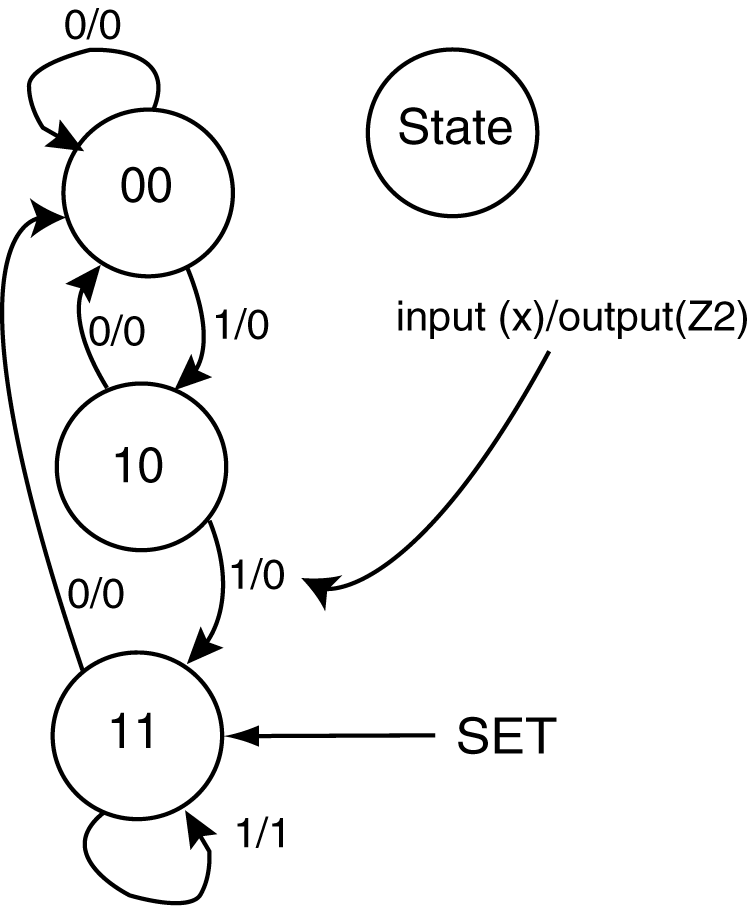
\includegraphics[width=5cm]{fsm/ex19.png}
\end{minipage}
\end{leftbar}
\noindent
\textbf{SOLUTION.} The state diagram shown in this problem indicates that this is a three-state FSM with one Mealy-type external output and one external input. Since there are three states, the solution requires at least two state variables to handle the three states. The black-box diagram of the solution is shown in Listing~\ref{exe_19_code}. Note that the two state variables are handled as a bundled signal.


\begin{figure}[!h]
    \centering
	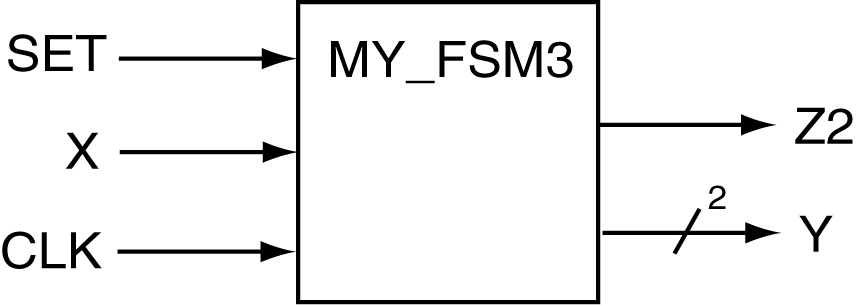
\includegraphics[width=5cm]{fsm/ex19_sol.png}
\end{figure}

\noindent
\begin{minipage}{0.99\linewidth}
\begin{lstlisting}[label=exe_19_code, caption=Solution to Example~19.]
-- library declaration
library IEEE;
use IEEE.std_logic_1164.all;
-- entity
entity my_fsm3 is 
    port ( X,CLK,SET : in  std_logic; 
                   Y : out std_logic_vector(1 downto 0); 
                  Z2 : out std_logic); 
end my_fsm3;
-- architecture
architecture fsm3 of my_fsm3 is
   type state_type is (ST0,ST1,ST2); 
   signal PS,NS : state_type; 
begin
   sync_proc: process(CLK,NS,SET)
   begin
      if (SET = '1') then 
         PS <= ST2; 
      elsif (rising_edge(CLK)) then 
         PS <= NS; 
      end if; 
   end process sync_proc; 

   comb_proc: process(PS,X)
   begin
      Z2 <= '0';           -- pre-assign FSM outputs
      case PS is 
         when ST0 =>       -- items regarding state ST0
            Z2 <= '0';     -- Mealy output always 0
            if (X = '0') then NS <= ST0;  
            else  NS <= ST1; 
            end if; 
         when ST1 =>       -- items regarding state ST1
            Z2 <= '0';     -- Mealy output always 0
            if (X = '0') then NS <= ST0; 
            else  NS <= ST2; 
            end if; 
         when ST2 =>       -- items regarding state ST2
            -- Mealy output handled in the if statement
            if (X = '0') then NS <= ST0; Z2 <= '0'; 
            else  NS <= ST2;  Z2 <= '1';     
            end if; 
         when others =>    -- the catch all condition
            Z2 <= '1'; NS <= ST0; 
      end case; 
   end process comb_proc; 
 
   -- faking some state variable outputs
   with PS select
      Y <= "00" when ST0, 
           "10" when ST1, 
           "11" when ST2, 
           "00" when others; 
end fsm3;
\end{lstlisting}
\end{minipage}

As usual, there are a couple of fun things to point out about the solution for Example~19. Most importantly, you should note the similarities between this solution and the previous solution. 

\begin{my_list}
\item The FSM has one Mealy-type output. The solution essentially treats this output as a Moore-type output in the first two \texttt{when} clauses of the \texttt{case} statement. In the final \texttt{when} clause, the Z2 output appears in both sections of the \texttt{if} statement. The fact the Z2 output is different in the context of state ST2 that makes it a Mealy-type output and therefore a Mealy-type FSM. 

\item When faking the state variable outputs (keeping in mind that the actual state variables are represented with enumeration types), two signals are required since the state diagram contains more than two states (and less than five states). The solution opted is to represent these outputs as a bundle which has the effect of slightly changing the form of the selected signal assignment statement appearing at the end of the architecture description. 
\end{my_list}

\begin{leftbar}
\begin{minipage}[t]{0.5\textwidth}
\vspace{10pt}
\noindent
\textbf{EXAMPLE 20.}
Write the VHDL code that implements the FSM shown on the right. Use a dependent PS/NS coding style in your implementation. Consider the listed state variables as output.
\end{minipage}
\begin{minipage}[t]{0.47\textwidth}
\vspace{0pt}\raggedright
\centering
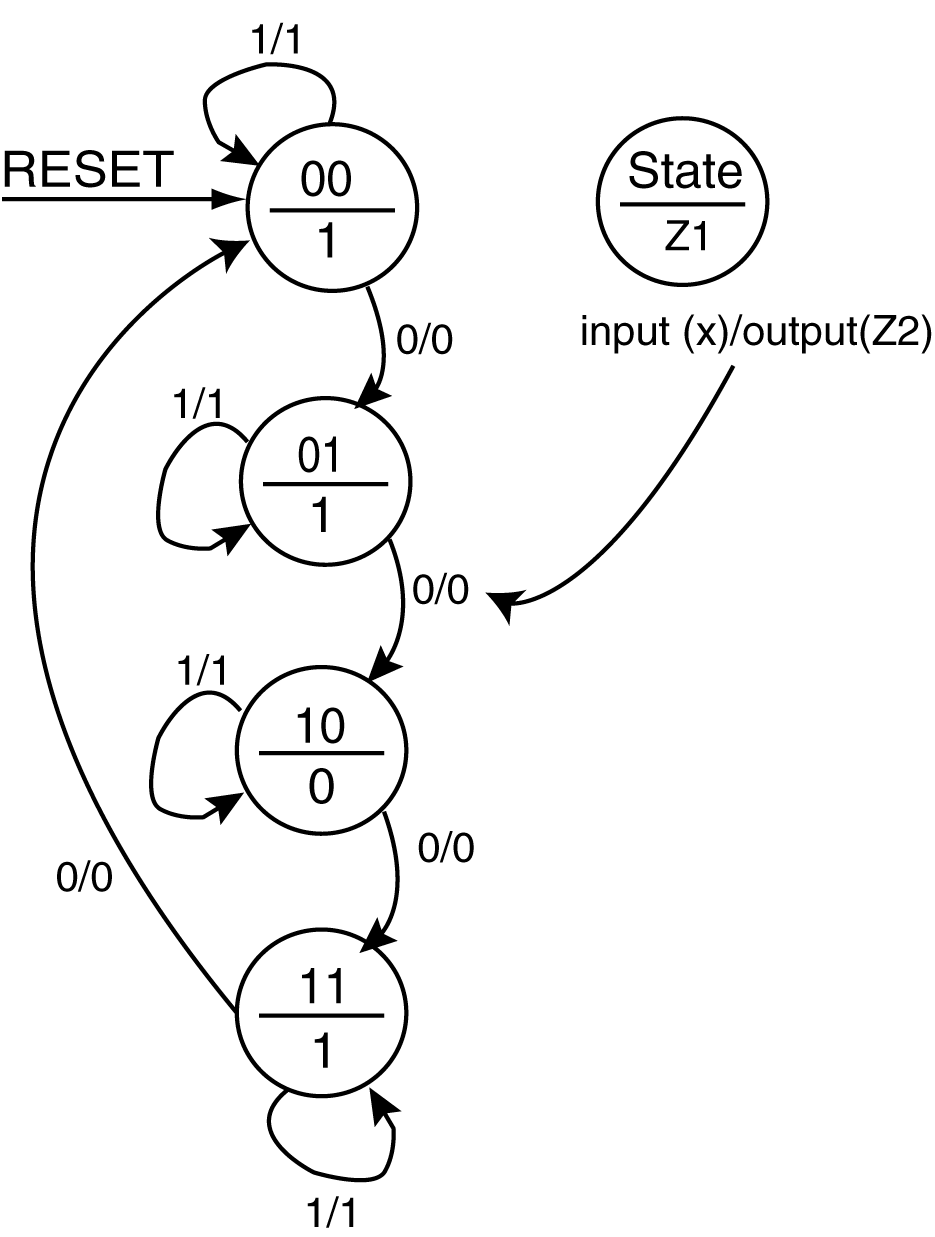
\includegraphics[width=5.2cm]{fsm/ex20.png}
\end{minipage}
\end{leftbar}

\noindent
\textbf{SOLUTION.} The state diagram indicates that its implementation will contain four states, one external input and two external outputs. This is a hybrid FSM in that the if contains both a Mealy and Moore-type output but in this case, the FSM would be considered a Mealy-type FSM. The black-box diagram and the actual solution for the solution is shown in Listing~\ref{exe_20_code}. 
\begin{figure}[!h]
    \centering
	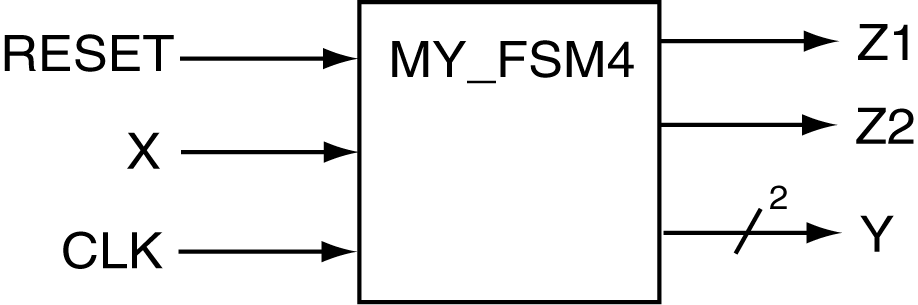
\includegraphics[width=5cm]{fsm/ex20_sol.png}
\end{figure}

\noindent
\begin{minipage}{0.99\linewidth}
\begin{lstlisting}[label=exe_20_code, caption=Solution to Example~20.]
-- library declaration
library IEEE;
use IEEE.std_logic_1164.all;
-- entity
entity my_fsm4 is 
    port ( X,CLK,RESET : in  std_logic; 
                     Y : out std_logic_vector(1 downto 0); 
                 Z1,Z2 : out std_logic);  
end my_fsm4;
-- architecture
architecture fsm4 of my_fsm4 is
   type state_type is (ST0,ST1,ST2,ST3); 
   signal PS,NS : state_type; 
begin
   sync_proc: process(CLK,NS,RESET)
   begin
     if (RESET = '1') then  PS <= ST0; 
     elsif (rising_edge(CLK)) then  PS <= NS; 
     end if; 
   end process sync_proc; 

   comb_proc: process(PS,X)
   begin
      -- Z1: the Moore output; Z2: the Mealy output
      Z1 <= '0';   Z2 <= '0'; -- pre-assign the outputs
      case PS is 
         when ST0 =>    -- items regarding state ST0
            Z1 <= '1';  -- Moore output 
            if (X = '0') then NS <= ST1; Z2 <= '0';   
            else  NS <= ST0; Z2 <= '1';
            end if; 
         when ST1 =>    -- items regarding state ST1
            Z1 <= '1';  -- Moore output 
            if (X = '0') then NS <= ST2; Z2 <= '0';  
            else  NS <= ST1; Z2 <= '1'; 
            end if; 
         when ST2 =>    -- items regarding state ST2
            Z1 <= '0';  -- Moore output 
            if (X = '0') then NS <= ST3; Z2 <= '0'; 
            else  NS <= ST2; Z2 <= '1'; 
            end if; 
         when ST3 =>    -- items regarding state ST3
            Z1 <= '1';  -- Moore output 
            if (X = '0') then NS <= ST0; Z2 <= '0'; 
            else  NS <= ST3;  Z2 <= '1';     
            end if; 
         when others => -- the catch all condition
            Z1 <= '1';  Z2 <= '0';  NS <= ST0; 
      end case; 
   end process comb_proc; 
 
   with PS select
      Y <= "00" when ST0, 
           "01" when ST1, 
           "10" when ST2, 
           "11" when ST3, 
           "00" when others; 
end fsm4;
\end{lstlisting}
\end{minipage}

If you haven't noticed by now, implementing FSMs using the VHDL behavioral model is remarkably straightforward. In reality, I rarely code a FSM from scratch; I usually opt to grab some previous FSM I have coded and start from there. Keep in mind that real engineering is rarely based on a cookbook. For FSM problems, the engineering is in the testing and creation of the state diagram. Do not get too comfortable with behavioral modeling of FSMs; the real fun is actually generating a FSM that solves a given problem. 

\section{One-Hot Encoding for FSMs}
Truth told, there are many different methods that can be used to encode state variables\footnote{In this case, encoding refers to the act of assigning a unique pattern of  1's and 0's to each of the state in order to make them unambiguous from other states.}. If the exact form of the representation used is important to you, then you will need to take the necessary steps in order to control how the state variables are represented by the synthesizer. There are two approaches to control state variable representation. The first approach is to allow the synthesizing tool to handle the details. Since every FSM we have seen up to this point has used enumeration types to represent the state variables, the synthesizer could choose to actually represent them with an encoding scheme of its own choosing. The reality is that the tools generally have an option to select the desired encoding scheme. The downside of this approach is that you are denied the learning experience associated with implementing the VHDL code that explicitly induces your desired encoding scheme. After all, you may have some special encoding scheme you need to use but is not supported by the development tools. The second approach to encoding the state variables is to specify them directly in VHDL. The approach of specifying the state variables in the VHDL code is presented in this section. 

One-hot encoding uses one bit in the state register for each state of the FSM. For a one-hot encoding FSM with 16 states, 16 flip flops are required. However only four flip flops are required if the same FSM is implemented using a binary encoding. One-hot encoding simplifies the logic and the interconnections between overall logic. Despite looking quite wasteful in terms of employed logic, one-hot encoding often results in smaller and faster FSMs.

The approach taken in the previous FSM examples was to pretend we were using full encoding for the state variables of the FSM. The full encoding approach minimizes the number of storage elements (flip-flops) used to store the state variables. The closed form equation describing the number of flip-flops required for a given FSM as a function of the number of states is shown in equation \ref{eq1}. The bracket-like symbols used in equation \ref{eq1} indicate a ceiling function\footnote{The ceiling function $y=\lceil x \rceil$ assigns $y$ to the smallest integer that is greater or equal to $x$.}. The binary nature expressed by this equation is so apparent that this encoding is often referred to as binary encoding.

\begin{equation}\label{eq1}
 \#(flip\_flops) = \lceil \log_2(\#states) \rceil
\end{equation}

For one-hot encoded FSMs, only one flip-flop is asserted at any given time. This requires that each distinct state be represented by one flip-flop. In one-hot encoding, the number of flip-flops required to implement a FSM is therefore equal to the number of states in the FSM. The closed form of this relationship is shown in equation \ref{eq2}. 

\begin{equation}\label{eq2}
 \#(flip\_flops) = \lceil \#(states) \rceil
\end{equation}

The question naturally arises as to how VHDL can be used to implement one-hot encoded FSMs. If you want total control of the process, you will need to grab control away from the synthesizer. And since we are concerned with learning VHDL, we need to look at the process of explicitly encoding one-hot FSMs. 

The modular approach we used to implement FSMs expedites the conversion process from using enumeration types to actually specifying how the state variables are represented. The changes from our previous approach are limited to how the outputs are assigned to the state variables and how the state variables are forced to be represented by certain bit patterns. Modifications to the fully encoded approach are thus limited to the entity declaration (you will need more variables to represent the states), the declaration of the state variables (you will need to explicitly declare the bit patterns associated with each state) and the assignment of the state variables to the outputs (in this case, we are actually not faking it like we were in other examples). 

\begin{leftbar}
\begin{minipage}[t]{0.5\textwidth}
\vspace{10pt}
\noindent
\textbf{EXAMPLE 21.}
Write the VHDL code that implements the FSM shown on the right. Use a dependent PS/NS coding style in your implementation. Consider the listed state variables as output. Use one-hot encoding for the state variables. This problem is Example~20 all over again but uses true one-hot encoding for the state variables. 
\vspace{50px}
\end{minipage}
\begin{minipage}[t]{0.47\textwidth}
\vspace{0pt}\raggedright
    \centering
	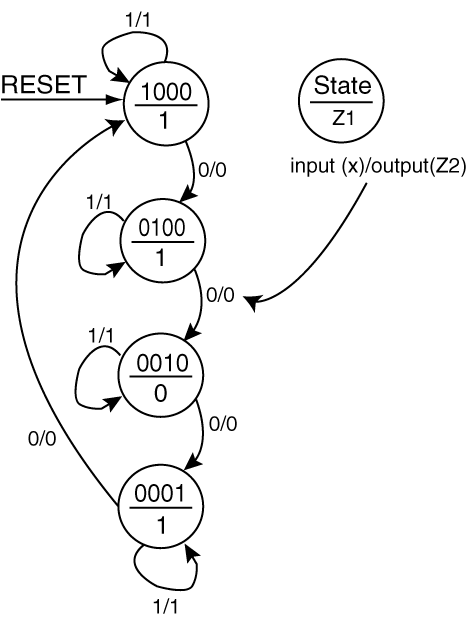
\includegraphics[width=5cm]{fsm/ex21.png}
\end{minipage}
\end{leftbar}
\noindent
\textbf{SOLUTION.} The state diagram shows four states, one external input X, two external outputs Z1 and Z2 with the Z2 output being a Mealy output. This is a Mealy machine that indicates one-hot encoding should be used to encode the state variables. We will approach the implementation of this FSM one piece at the time.

Listing~\ref{exe_21_code_1} shows the modifications to the entity declaration required to convert the full encoding used in Example~20 to a pseudo one-hot encoding. Listing~\ref{exe_21_code_2} shows the required modifications to the state variable output assignment in order to move from enumeration types to a special form of assigned types. Forcing the state variables to be truly encoded using one-hot encoding requires these two extra lines of code as is shown in Listing~\ref{exe_21_code_2}. These two lines of code essentially force the VHDL synthesizer to represent each state of the FSM with its own storage element. In other words, each state is represented by the "string" modifier as listed. This forces four bits per state to be remembered by the FSM implementation which essentially requires four flip-flops. Note in Listing~\ref{exe_21_code_3} that the default case is assigned a valid one-hot state instead of the customary all zero state. You should strongly consider comparing these three figures. The total solution is shown in Listing~\ref{exe_21_code_4} 

\noindent
\begin{minipage}{0.99\linewidth}
\begin{lstlisting}[label=exe_21_code_1, caption=Modifications to convert Example~20 to one-hot encoding.]
-- full encoded approach
entity my_fsm4 is 
    port ( X,CLK,RESET : in  std_logic; 
                     Y : out std_logic_vector(1 downto 0); 
                 Z1,Z2 : out std_logic);  
end my_fsm4;
----------------------------------------------------------------------
-- one-hot encoding approach
entity my_fsm4 is 
    port ( X,CLK,RESET : in  std_logic; 
                     Y : out std_logic_vector(3 downto 0); 
                 Z1,Z2 : out std_logic);  
end my_fsm4;
\end{lstlisting}

\begin{lstlisting}[label=exe_21_code_2, caption=Modifications to convert state variables to use one-hot encoding.]
-- the approach for enumeration types   
type state_type is (ST0,ST1,ST2,ST3); 
signal PS,NS : state_type; 
----------------------------------------------------------------------
-- the approach used for explicitly specifying state bit patterns
type state_type is (ST0,ST1,ST2,ST3); 
attribute ENUM_ENCODING: STRING; 
attribute ENUM_ENCODING of state_type: type is "1000 0100 0010 0001";
signal PS,NS : state_type;
\end{lstlisting}
\end{minipage}

\noindent
\begin{minipage}{0.99\linewidth}
\begin{lstlisting}[label=exe_21_code_3, caption=Modifications to convert state output to pseudo one-hot encoding.]
-- fake full encoded approach 
with PS select
   Y <= "00" when ST0, 
        "01" when ST1, 
        "10" when ST2, 
        "11" when ST3, 
        "00" when others; 
end fsm4;
----------------------------------------------------------------------
-- one-hot encoded approach 
with PS select
   Y <= "1000" when ST0, 
        "0100" when ST1, 
        "0010" when ST2, 
        "0001" when ST3, 
        "1000" when others; 
end fsm4;
\end{lstlisting}
\end{minipage}

\noindent
\begin{minipage}{0.99\linewidth}
\begin{lstlisting}[label=exe_21_code_4, caption=The final solution to Example~21.]
-- library declaration
library IEEE;
use IEEE.std_logic_1164.all;
-- entity
entity my_fsm4_oh is 
    port ( X,CLK,RESET : in  std_logic; 
                     Y : out std_logic_vector(3 downto 0); 
                 Z1,Z2 : out std_logic);  
end my_fsm4_oh;
-- architeture
architecture fsm4_oh of my_fsm4_oh is
  type state_type is (ST0,ST1,ST2,ST3);
  attribute ENUM_ENCODING: STRING; 
  attribute ENUM_ENCODING of state_type: type is "1000 0100 0010 0001";
  signal PS,NS : state_type; 
begin
   sync_proc: process(CLK,NS,RESET)
   begin
     if (RESET = '1') then  PS <= ST0; 
     elsif (rising_edge(CLK)) then  PS <= NS; 
     end if; 
   end process sync_proc; 

   comb_proc: process(PS,X)
   begin
      -- Z1: the Moore output; Z2: the Mealy output
      Z1 <= '0';   Z2 <= '0'; -- pre-assign the outputs
      case PS is 
         when ST0 =>    -- items regarding state ST0
            Z1 <= '1';  -- Moore output 
            if (X = '0') then NS <= ST1; Z2 <= '0';   
            else  NS <= ST0; Z2 <= '1';
            end if; 
         when ST1 =>    -- items regarding state ST1
            Z1 <= '1';  -- Moore output 
            if (X = '0') then NS <= ST2; Z2 <= '0';  
            else  NS <= ST1; Z2 <= '1'; 
            end if; 
         when ST2 =>    -- items regarding state ST2
            Z1 <= '0';  -- Moore output 
            if (X = '0') then NS <= ST3; Z2 <= '0'; 
            else  NS <= ST2; Z2 <= '1'; 
            end if; 
         when ST3 =>    -- items regarding state ST3
            Z1 <= '1';  -- Moore output 
            if (X = '0') then NS <= ST0; Z2 <= '0'; 
            else  NS <= ST3;  Z2 <= '1';     
            end if; 
         when others => -- the catch all condition
            Z1 <= '1';  Z2 <= '0';  NS <= ST0; 
      end case; 
   end process comb_proc; 
 
   -- one-hot encoded approach 
   with PS select
      Y <= "1000" when ST0, 
           "0100" when ST1, 
           "0010" when ST2, 
           "0001" when ST3, 
           "1000" when others; 

end fsm4_oh;
\end{lstlisting}
\end{minipage}

\section{Important Points}

\begin{my_list}
\item Modeling FSMs from a state diagram is a straightforward process using VHDL behavioral modeling. The process is so straightforward that it is often considered cookie cutter. The real engineering involved in implementing FSM is in the generation of the state diagram that solved the problem at hand.

\item Due to the general versatility of VHDL, there are many approaches that can be used to model FSMs using VHDL. The approach used here details only one of those styles but is generally considered the most straightforward of all styles. 

\item The actual encoding of the FSM's state variables when enumeration types are used is left up to the synthesis tool. If a preferred method of variable encoding is desired, using the attribute approach detail in this section is a simple but viable alternative. 
\end{my_list}

\section{Exercises: Behavioral Modeling of FSMs}

%%%%%% EXERCISE 1 %%%%%%
\vspace{20pt}
\noindent
\begin{minipage}{1\textwidth}
\textbf{EXERCISE 1.}
Draw the state diagram associated with the following VHDL code. Be sure to provide a legend and completely label everything.
\end{minipage}
\begin{minipage}{0.66\textwidth}
\vspace{10px}
\begin{lstlisting}
-- library declaration
library IEEE;
use IEEE.std_logic_1164.all;
-- entity
entity fsm is 
   port (  X,CLK : in  std_logic; 
           RESET : in  std_logic; 
           Z1,Z2 : out std_logic;  
end fsm;
-- architecture
architecture fsm of fsm is
   type state_type is (A,B,C);
   signal PS,NS : state_type;
begin
   sync_proc: process(CLK,NS,RESET)
   begin
      if (RESET = '0') then PS <= C; 
      elsif (rising_edge(CLK)) then PS <= NS; 
      end if; 
   end process sync_proc; 

   comb_proc: process(PS,X)
   begin
      case PS is 
         Z1 <= '0';    Z2 <= '0'; 
         when A =>    
            Z1 <= '0';  
            if (X='0') then NS<=A; Z2<='1';   
            else  NS <= B; Z2 <= '0';
            end if; 
         when B =>    
            Z1 <= '1';  
            if (X='0') then NS<=A; Z2<='0';  
            else  NS <= C; Z2 <= '1'; 
            end if; 
         when C =>    
            Z1 <= '1';  
            if (X='0') then NS<=B; Z2<='1'; 
            else  NS <= A; Z2 <= '0'; 
            end if; 
         when others =>    
            Z1 <= '1'; NS<=A; Z2<='0'; 
      end case; 
   end process comb_proc; 
end fsm;
\end{lstlisting}
\end{minipage}
\begin{minipage}{0.29\textwidth}
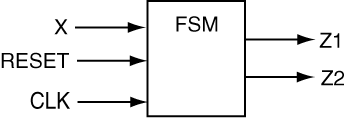
\includegraphics[width=4cm]{fsm/sm_ex1.png}
\vspace{250px}
\end{minipage}

%%%%%% EXERCISE 2 %%%%%%
\vspace{20pt}
\noindent
\begin{minipage}[t]{0.5\textwidth}
\textbf{EXERCISE 2.}
Write a VHDL behavioral model that could be used to implement the state diagram as shown on the right. The state variables should be encoded as listed and also provided as outputs of the FSM.
\end{minipage}
\begin{minipage}[t]{0.47\textwidth}
\vspace{0pt}\raggedright
\centering
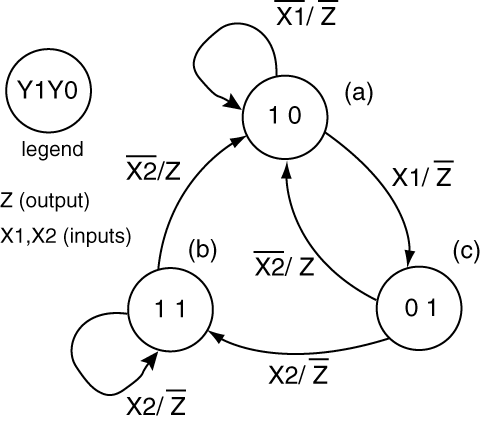
\includegraphics[width=5.3cm]{fsm/sm_ex2.png}
\end{minipage}

%%%%%% EXERCISE 3 %%%%%%
\vspace{20pt}
\noindent
\begin{minipage}{1\textwidth}
\textbf{EXERCISE 3.}
Draw the state diagram associated with the following VHDL code. Be sure to provide a legend and remember to label everything.
\end{minipage}
\begin{minipage}{0.66\textwidth}
\vspace{10px}
\begin{lstlisting}
-- library declaration
library IEEE;
use IEEE.std_logic_1164.all;
-- entity
entity fsmx is
    Port ( BUM1,BUM2 : in  std_logic;
                 CLK : in   std_logic;
            TOUT,CTA : out std_logic);
end fsmx;
-- architecture
architecture my_fsmx of fsmx is
   type state_type is (S1,S2,S3); 
	signal PS,NS : state_type; 
begin
   sync_p: process (CLK,NS)
   begin
      if (rising_edge(CLK)) then   
         PS <= NS; 
      end if; 
   end process sync_p; 

   comb_p: process (CLK,BUM1,BUM2)
   begin
      case PS is 

         when S1 => 
            CTA <= '0'; 
            if (BUM1 = '0')  then 
               TOUT <= '0'; 
               NS <= S1; 
            elsif (BUM1 = '1') then 
               TOUT <= '1';  
               NS <= S2; 
            end if; 

         when S2 =>
            CTA <= '0'; 
            TOUT <= '0'; 
            NS <= S3;   

         when S3 =>
            CTA <= '1'; 
            TOUT <= '0';   
            if (BUM2 = '1')  then 
               NS <= S1; 
            elsif (BUM2 = '0') then 
               NS <= S2; 
            end if; 
      
         when others =>   CTA <= '0'; 
                         TOUT <= '0';
                           NS <= S1;
      end case; 
   end process comb_p; 
end my_fsmx;
\end{lstlisting}
\end{minipage}
\begin{minipage}{0.29\textwidth}
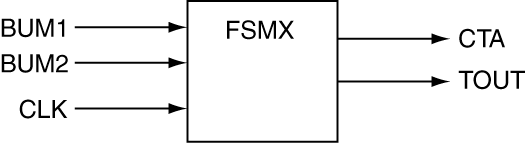
\includegraphics[width=4cm]{fsm/sm_ex3.png}
\vspace{250px}
\end{minipage}

%%%%%% EXERCISE 4 %%%%%%
\vspace{20pt}
\noindent
\begin{minipage}[t]{0.5\textwidth}
\textbf{EXERCISE 4.}
Write the VHDL behavioral model code that could be used to implement the state diagram on shown in the right.
\end{minipage}
\begin{minipage}[t]{0.47\textwidth}
\vspace{0pt}\raggedright
\centering
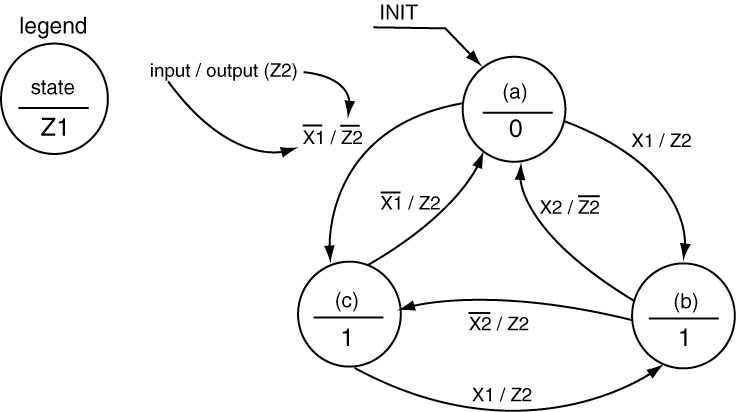
\includegraphics[width=5.7cm]{fsm/sm_ex4.png}
\end{minipage}

%%%%%% EXERCISE 5 %%%%%%
\vspace{20pt}
\noindent
\begin{minipage}{1\textwidth}
\textbf{EXERCISE 5.}
Draw the state diagram associated with the following VHDL code. Consider the outputs \texttt{Y} to be representative of the state variables. Be sure to provide a legend. Indicate the states with both state variables and their symbolic equivalents.
\end{minipage}
\begin{minipage}{1\textwidth}
\vspace{10px}
\begin{lstlisting}
-- library declaration
library IEEE;
use IEEE.std_logic_1164.all;
-- entity
entity fsm is 
port (     X,CLK : in  std_logic; 
           RESET : in  std_logic; 
           Z1,Z2 : out std_logic;  
               Y : out std_logic_vector(2 downto 0)); 
end fsm;
-- architecture
architecture my_fsm of fsm is
   type state_type is (A,B,C);
   attribute ENUM_ENCODING: STRING; 
   attribute ENUM_ENCODING of state_type: type is "001 010 100";
   signal PS,NS : state_type;
begin

sync_proc: process(CLK,NS,RESET) -- process
   begin
     if (RESET = '0') then PS <= C; 
     elsif (rising_edge(CLK)) then PS <= NS; 
     end if; 
   end process sync_proc; 

comb_proc: process(PS,X) -- process
   begin
      case PS is 
         when A =>    
            Z1 <= '0';  
            if (X = '0') then NS <= A; Z2 <= '1';   
            else  NS <= B; Z2 <= '0';
            end if; 
         when B =>    
            Z1 <= '1';  
            if (X = '0') then NS <= A; Z2 <= '0';  
            else  NS <= C; Z2 <= '1'; 
            end if; 
         when C =>    
            Z1 <= '1';  
            if (X = '0') then NS <= B; Z2 <= '1'; 
            else  NS <= A; Z2 <= '0'; 
            end if; 
         when others =>    
            Z1 <= '1'; NS <= A; Z2 <= '0';  
      end case; 
   end process comb_proc; 
 
with PS select
   Y <= "001" when A, 
        "010" when B, 
        "100" when C, 
        "001" when others; 
end my_fsm;
\end{lstlisting}
\end{minipage}

%%%%%% EXERCISE 6 %%%%%%
\vspace{20pt}
\noindent
\begin{minipage}[t]{0.5\textwidth}
\textbf{EXERCISE 6.}
Write a VHDL behavioral model code that can be used to implement the state diagram shown on the right. All state variables should be encoded as listed and also provided as outputs of the FSM.
\end{minipage}
\begin{minipage}[t]{0.47\textwidth}
\vspace{0pt}\raggedright
\centering
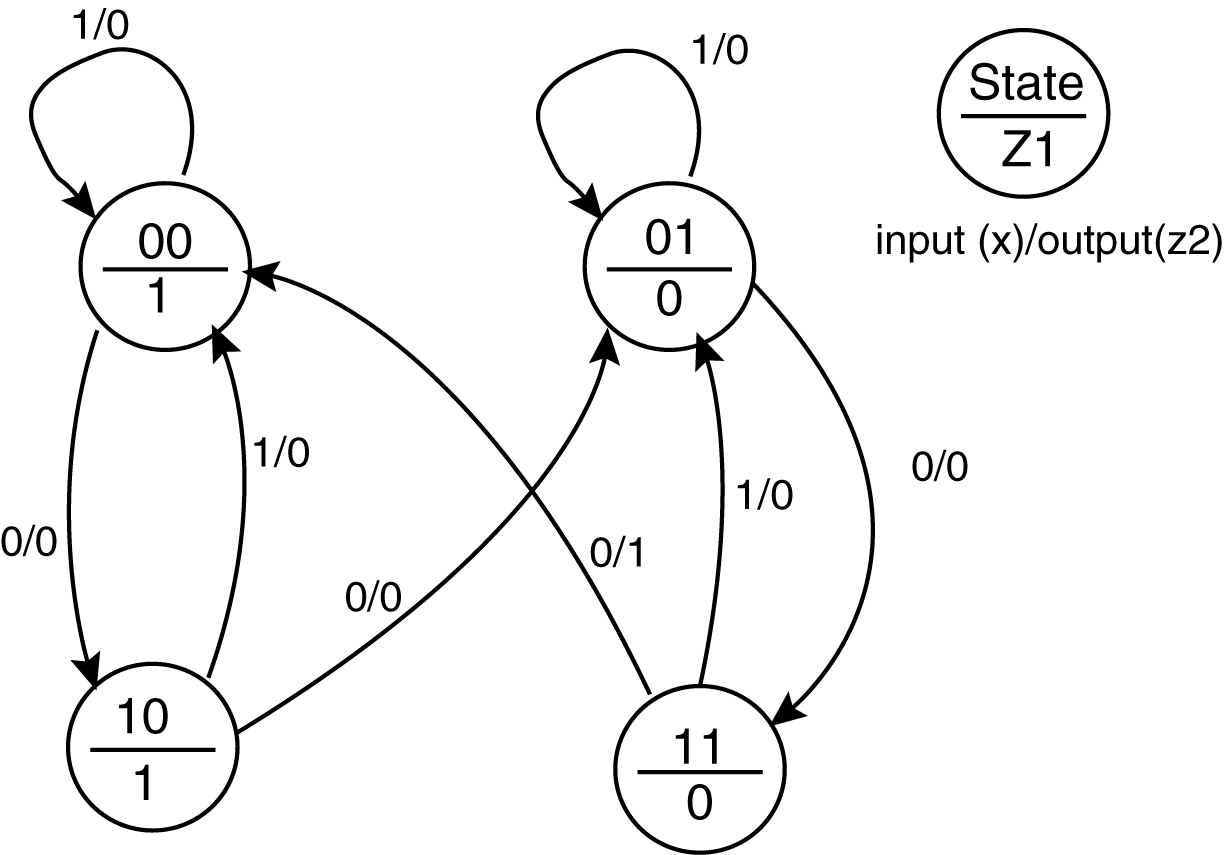
\includegraphics[width=6cm]{fsm/sm_ex6.png}
\end{minipage}

%%%%%% EXERCISE 7 %%%%%%
\vspace{20pt}
\noindent
\begin{minipage}{1\textwidth}
\textbf{EXERCISE 7.}
Draw the state diagram that corresponds to the following VHDL model and state whether the FSM is a Mealy machine or a Moore machine. Be sure to label everything.
\vspace{10pt}
\end{minipage}
\begin{minipage}{0.66\textwidth}

\begin{lstlisting}
-- library declaration
library IEEE;
use IEEE.std_logic_1164.all;
-- entity
entity fsm is
    Port ( CLK,CLR,SET,X1,X2 : in  std_logic;
                       Z1,Z2 : out std_logic);
end fsm;
-- architecture
architecture my_fsm of fsm is
   type state_type is (sA,sB,sC,sD); 
   attribute ENUM_ENCODING: STRING; 
   attribute ENUM_ENCODING of state_type: type is "1000 0100 0010 0001";
   signal PS,NS : state_type; 
begin
   sync_p: process (CLK,NS,CLR,SET) -- process
   begin
      if (CLR = '1' and SET = '0') then 
         PS <= sA; 
	  elsif (CLR = '0' and SET = '1') then 
	     PS <= sD;
      elsif (rising_edge(CLK)) then   
         PS <= NS; 
      end if; 
   end process sync_p; 

   comb_p: process (X1,X2,PS) -- process
   begin
      case PS is 
         when sA =>  
            if ( X1 = '1')  then 
               Z1 <= '0'; Z2 <= '0';   
               NS <= sA; 
            else  
               Z1 <= '0'; Z2 <= '0';   
               NS <= sB; 
            end if; 
         when sB =>
            if ( X2 = '1')  then 
               Z1 <= '1'; Z2 <= '1';   
               NS <= sC; 
            else  
               Z1 <= '1'; Z2 <= '0';   
               NS <= sB; 
            end if;				
         when sC =>
            if ( X2 = '1')  then 
               Z1 <= '0'; Z2 <= '0';   
               NS <= sB; 
            else  
               Z1 <= '0'; Z2 <= '1';   
               NS <= sC; 
            end if;
         when sD =>
            if ( X1 = '1')  then 
               Z1 <= '1'; Z2 <= '1';   
               NS <= sD; 
            else  
               Z1 <= '1'; Z2 <= '1';   
               NS <= sC; 
            end if;				
      end case; 
   end process comb_p; 
end my_fsm;
\end{lstlisting}
\end{minipage}
\begin{minipage}{0.29\textwidth}
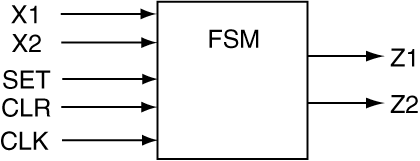
\includegraphics[width=4cm]{fsm/sm_ex7.png}
\vspace{250px}
\end{minipage}

%%%%%% EXERCISE 8 %%%%%%
\vspace{20pt}
\noindent
\begin{minipage}[t]{0.5\textwidth}
\textbf{EXERCISE 8.}
Write the VHDL behavioral model code that can be used to implement the state diagram shown on the right. The state variables should be encoded as listed and also provided as outputs of the FSM.
\end{minipage}
\begin{minipage}[t]{0.47\textwidth}
\vspace{0pt}\raggedright
\centering
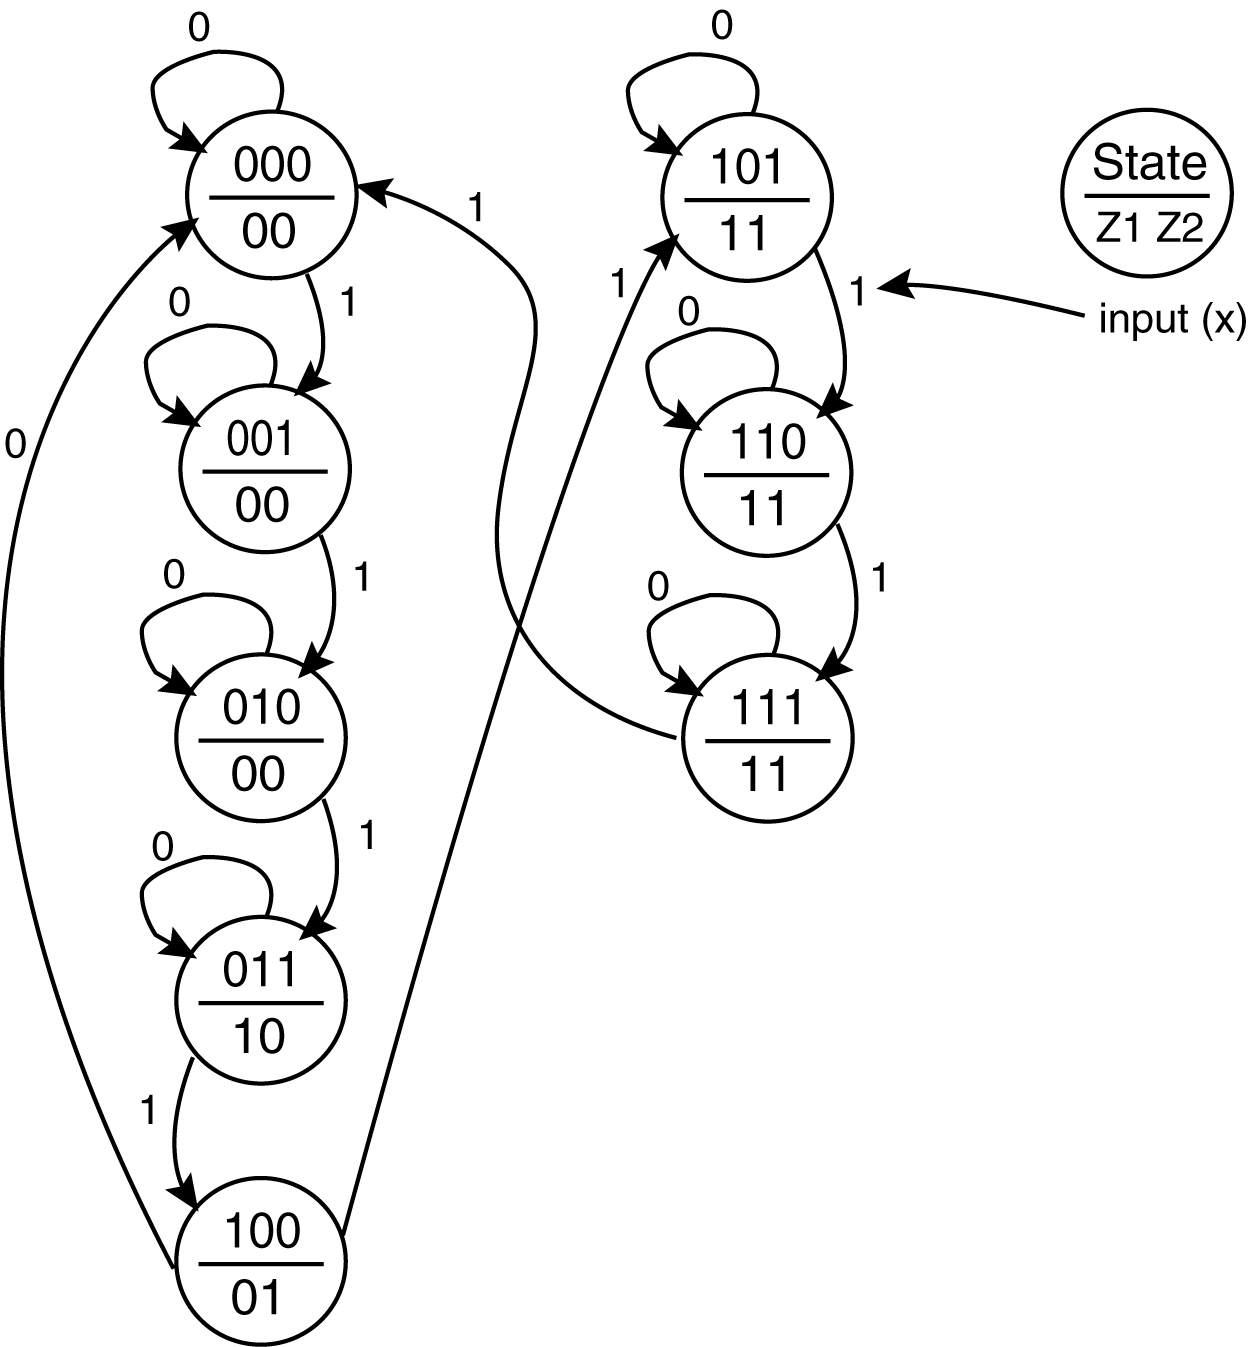
\includegraphics[width=5.3cm]{fsm/sm_ex8.png}
\end{minipage}

%%%%%% EXERCISE 9 %%%%%%
\vspace{20pt}
\noindent
\begin{minipage}[t]{0.5\textwidth}
\textbf{EXERCISE 9.}
Write the VHDL behavioral model code that can be used to implement the state diagram shown on the right. The state variables should be encoded as listed and also provided as outputs of the FSM.
\end{minipage}
\begin{minipage}[t]{0.47\textwidth}
\vspace{0pt}\raggedright
\centering
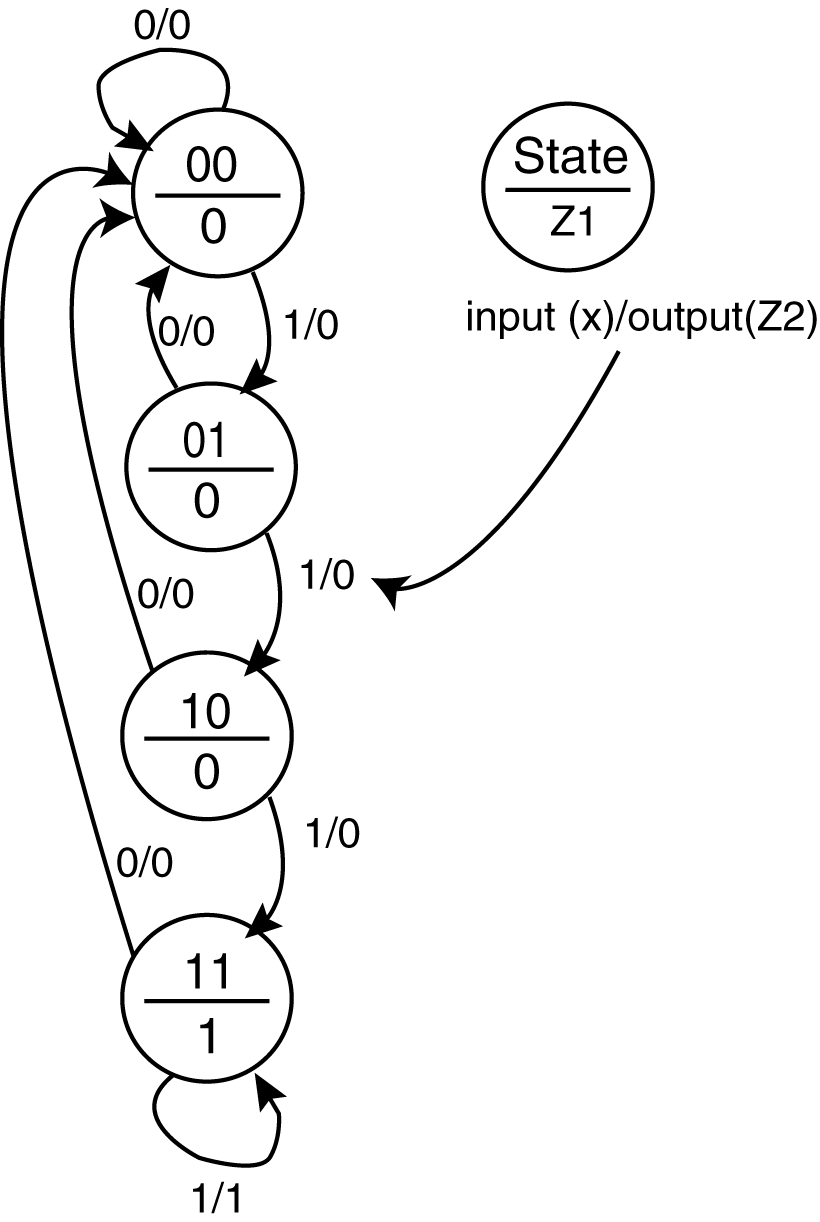
\includegraphics[width=4.2cm]{fsm/sm_ex9.png}
\end{minipage}

%%%%%% EXERCISE 10 %%%%%%
\vspace{20pt}
\noindent
\begin{minipage}[t]{0.5\textwidth}
\textbf{EXERCISE 10.}
Write the VHDL behavioral model code that can be used to implement the state diagram shown on the right. The state variables should be encoded as listed and also provided as outputs of the FSM.
\end{minipage}
\begin{minipage}[t]{0.47\textwidth}
\vspace{0pt}\raggedright
\centering
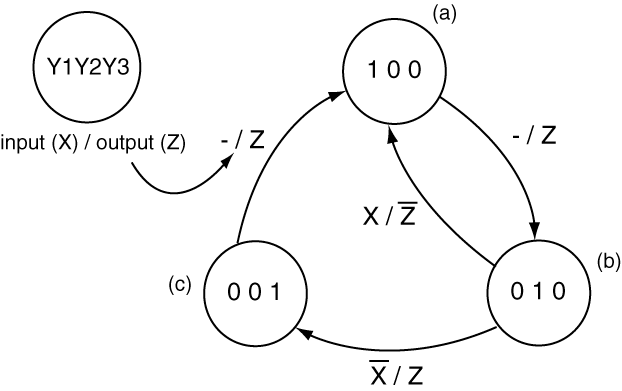
\includegraphics[width=6cm]{fsm/sm_ex10.png}
\end{minipage}

%%%%%% EXERCISE 11 %%%%%%
\vspace{20pt}
\noindent
\begin{minipage}[t]{0.5\textwidth}
\textbf{EXERCISE 11.}
Write the VHDL behavioral model code that can be used to implement the state diagram shown on the right. The state variables should be encoded as listed and also provided as outputs of the FSM.
\end{minipage}
\begin{minipage}[t]{0.47\textwidth}
\vspace{0pt}\raggedright
\centering
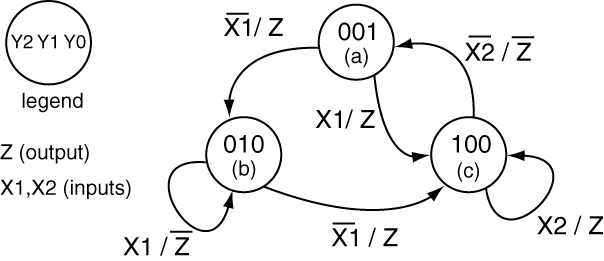
\includegraphics[width=6.4cm]{fsm/sm_ex11.png}
\end{minipage}

%%%%%% EXERCISE 12 %%%%%%
\vspace{20pt}
\noindent
\begin{minipage}[t]{1\textwidth}
\textbf{EXERCISE 12.}
Write the VHDL behavioral model code that can be used to implement the state diagram shown on the right. The state variables should be encoded as listed and also provided as outputs of the FSM.
\end{minipage}
\begin{minipage}[t]{1\textwidth}
\vspace{10pt}
\centering
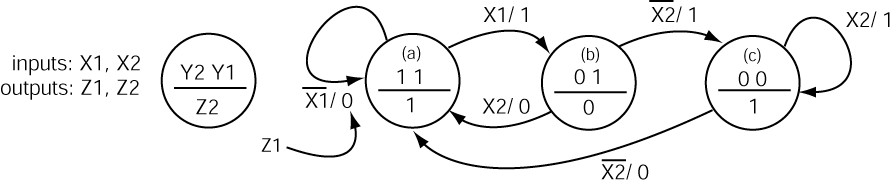
\includegraphics[width=11cm]{fsm/sm_ex12.png}
\end{minipage}

%%%%%% EXERCISE 13 %%%%%%
\vspace{20pt}
\noindent
\begin{minipage}[t]{0.5\textwidth}
\textbf{EXERCISE 13.}
Write the VHDL behavioral model code that can be used to implement the state diagram shown on the right. The state variables should be encoded as listed and also provided as outputs of the FSM.
\end{minipage}
\begin{minipage}[t]{0.47\textwidth}
\vspace{0pt}\raggedright
\centering
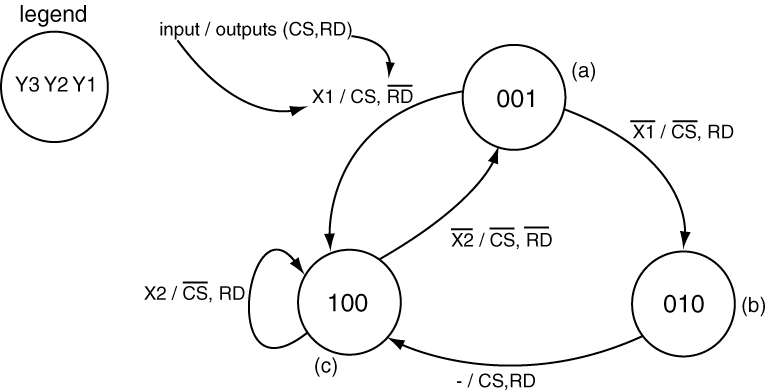
\includegraphics[width=6cm]{fsm/sm_ex13.png}
\end{minipage}

%%%%%% EXERCISE 14 %%%%%%
\vspace{20pt}
\noindent
\begin{minipage}[t]{0.5\textwidth}
\textbf{EXERCISE 14.}
Write the VHDL behavioral model code that can be used to implement the state diagram shown on the right. The state variables should be encoded as listed and also provided as outputs of the FSM.
\end{minipage}
\begin{minipage}[t]{0.47\textwidth}
\vspace{0pt}\raggedright
\centering
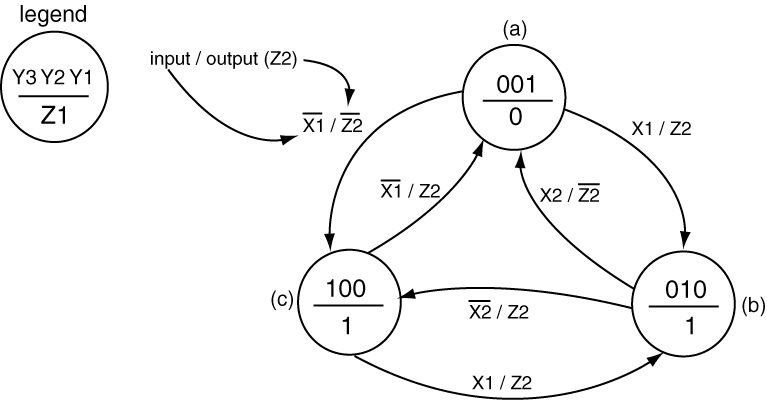
\includegraphics[width=6cm]{fsm/sm_ex14.png}
\end{minipage}



